%
% $RCSfile: systems_interconnection.tex,v $
%
% Copyright (C) 2002-2008. Christian Heller.
%
% Permission is granted to copy, distribute and/or modify this document
% under the terms of the GNU Free Documentation License, Version 1.1 or
% any later version published by the Free Software Foundation; with no
% Invariant Sections, with no Front-Cover Texts and with no Back-Cover
% Texts. A copy of the license is included in the section entitled
% "GNU Free Documentation License".
%
% http://www.cybop.net
% - Cybernetics Oriented Programming -
%
% http://www.resmedicinae.org
% - Information in Medicine -
%
% Version: $Revision: 1.1 $ $Date: 2008-08-19 20:41:09 $ $Author: christian $
% Authors: Christian Heller <christian.heller@tuxtax.de>
%

\section{Systems Interconnection}
\label{systems_interconnection_heading}
\index{Systems Interconnection}
\index{Open Systems Interconnection}
\index{OSI}
\index{International Organization for Standardization}
\index{ISO OSI Reference Model}
\index{Simple Mail Transfer Protocol}
\index{SMTP}
\index{Telephone Network}
\index{Telnet}
\index{File Transfer Protocol}
\index{FTP}
\index{Hypertext Transfer Protocol}
\index{HTTP}
\index{Domain Name Service}
\index{DNS}
\index{X.226}
\index{Remote Procedure Call}
\index{RPC}
\index{Network Basic Input/ Output System}
\index{NetBIOS}
\index{Transfer Control Protocol}
\index{TCP}
\index{User Datagram Protocol}
\index{UDP}
\index{Transport Protocol Class 4}
\index{TP4}
\index{Sequence Package Exchange}
\index{SPX}
\index{Internet Protocol}
\index{IP}
\index{Internet Packet Exchange}
\index{IPX}
\index{Point-to-Point Protocol}
\index{PPP}
\index{Serial Line Internet Protocol}
\index{SLIP}
\index{Frame Relay}
\index{FR}
\index{X.25}
\index{Ethernet}
\index{Token Ring}
\index{Fiber Distributed Data Interface}
\index{FDDI}
\index{Ontology}
\index{Health Level Seven}
\index{HL7}
\index{TCP/IP}
\index{Universal Interactive Executive}
\index{UNIX}
\index{Operating System}
\index{OS}

Communication is essential to an IT environment as described before. To enable
and ease communication across different systems, special solutions have been
developed and accepted as \emph{de facto} or \emph{de jure} standards. One such
specification is the well-known \emph{Open Systems Interconnection} (OSI)
reference model, defined by the \emph{International Organization for Standardization}
(ISO). Numerous books \cite{tanenbaum2000} and documents on the web
\cite{payer} describe this model and its protocols.

\begin{figure}[ht]
    \begin{center}
        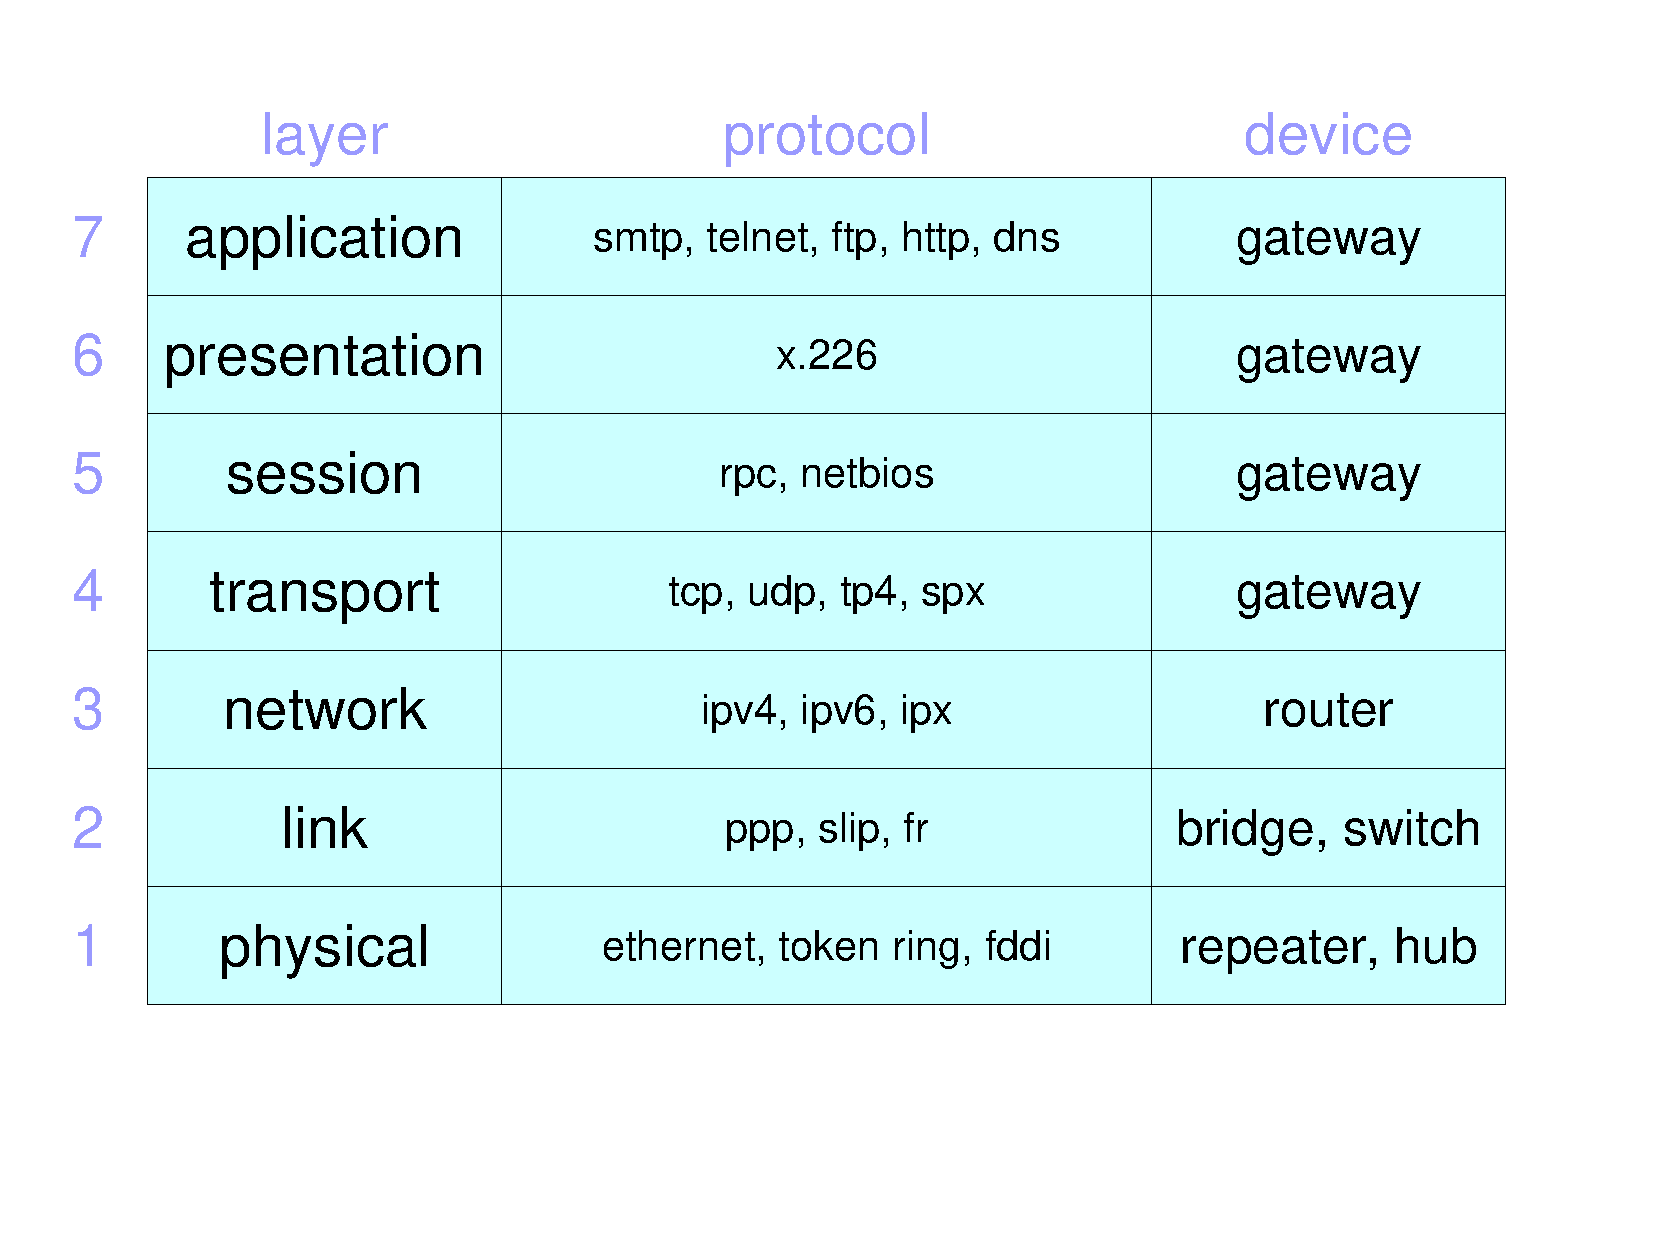
\includegraphics[scale=0.3,angle=-90]{graphic/osi.pdf}
        \caption{ISO OSI Reference Model}
        \label{osi_figure}
    \end{center}
\end{figure}

Figure \ref{osi_figure} organises the seven layers of the model in table form,
with one row representing one layer. The first column contains a layer's name,
the second examples of typical network protocols and the third devices in which
the protocols are used. \emph{Simple Mail Transfer Protocol} (SMTP),
\emph{Telephone Network} (Telnet), \emph{File Transfer Protocol} (FTP),
\emph{Hypertext Transfer Protocol} (HTTP) and \emph{Domain Name Service} (DNS)
are standard protocols used directly in software applications and -tools.
\emph{X.226} is a recommendation defining the OSI presentation protocol. The
\emph{Remote Procedure Call} (RPC) and \emph{Network Basic Input/ Output System}
(NetBIOS) may be sorted into the session layer. \emph{Transfer Control Protocol}
(TCP), \emph{User Datagram Protocol} (UDP), \emph{Transport Protocol Class 4}
(TP4) and \emph{Sequence Package Exchange} (SPX) do belong to the transport
layer. The \emph{Internet Protocol} (IP) is used in two versions: 4 and 6. Both
of them are situated on the network level of the OSI model, just like the
\emph{Internet Packet Exchange} (IPX) protocol. The link level contains the
\emph{Point-to-Point Protocol} (PPP), \emph{Serial Line Internet Protocol}
(SLIP) and \emph{Frame Relay} (FR), the latter being a replacement for veterans
like \emph{X.25}. To the physical level transmitting raw Bits finally, belong
\emph{Ethernet}, \emph{Token Ring} and \emph{Fiber Distributed Data Interface}
(FDDI).

Many of the mentioned protocols may be assigned to more than just one layer.
But it is \emph{not} the intention of this work to deal with such details. The
overall ISO OSI model, however, is mentioned because it is a good example of a
structure whose layers represent increasing levels of abstraction, what will
later in this work be called an \emph{Ontology} (chapters
\ref{logical_architecture_heading} and \ref{knowledge_schema_heading}). Also,
the \emph{Health Level Seven} (HL7) medical standard, which gets introduced in
chapter \ref{res_medicinae_heading}, received its name from referring to OSI's
seventh level -- the application level \cite{rogers}.

While the ISO OSI model defines seven abstract communication layers, the
popular \emph{TCP/IP} model uses solely four. Web communication as described in
section \ref{web_client_and_server_heading} is based on it. Today, TCP/IP has
become the standard in network management systems. A majority of them run the
\emph{Universal Interactive Executive} (UNIX) \emph{Operating System} (OS), of
which TCP/IP is an integral part. Margarete Payer \cite{payer} writes:
\textit{Although the OSI Model is affected with various deficiencies, it is
well suitable for didactic purposes.} Further, she mentions that since some
time, Andrew S. Tanenbaum uses a hybrid model for structuring his standard book
on computer networks \cite{tanenbaum2000}, which sticked to neither OSI nor
TCP/IP.
